\section{Butterfly as a worked derivation: why extra structure is necessary}
\label{sec:butterfly}

The butterfly is especially instructive because its first calculation can look like generic low-rank compression, while its speed comes from a second piece of organization. Start with
\begin{equation}
 K(x,\xi)=e^{2\pi i\Phi(x,\xi)},\qquad f=Kg.
 \label{eq:fiokernel}
\end{equation}
Rows correspond to positions $x$, columns to frequencies $\xi$. We follow Li, Yang, Martin, Ho and Ying's \emph{Butterfly Factorization} \cite{li2015butterfly}, while placing each construction step into the shared grammar.

\subsection{Two trees and the mixed phase}
There is no reason to use the same hierarchy for both variables: positions and frequencies have different roles. Let a tile have centers $(x_0,\xi_0)$ and define its nonseparable remainder by
\[
R(x,\xi)=\Phi(x,\xi)-\Phi(x,\xi_0)-\Phi(x_0,\xi)+\Phi(x_0,\xi_0).
\]
Then exactly
\begin{equation}
 e^{2\pi i\Phi(x,\xi)}
 =e^{2\pi i\Phi(x,\xi_0)}e^{2\pi iR(x,\xi)}
 e^{2\pi i(\Phi(x_0,\xi)-\Phi(x_0,\xi_0))}.
 \label{eq:phasepeel}
\end{equation}
The two one-variable factors are diagonal row and column scalings: they cannot change singular values or rank. Only the mixed remainder controls how many local patterns are required. If $\left|\partial_x\partial_\xi\Phi\right|\leq M$ and tile widths are $w_A,w_B$, the mixed-difference bound is
\begin{equation}
 |R(x,\xi)|\leq \frac{M}{4}w_Aw_B.
 \label{eq:phasebound}
\end{equation}
For the bilinear phase $\Phi=x\xi$, $R=(x-x_0)(\xi-\xi_0)$, so $\exp(2\pi iR)$ has a converging separated exponential series. Hence a small tile area gives a short sum in a completely explicit calculation.

For a general phase, this motivates what to measure; it does not replace the rank theorem's additional smoothness/analyticity hypotheses \cite{candes2009butterfly}. ``One phase-space cell has rank one'' is intuition; the peeled mixed phase is the rigorous object.

\subsection{Complementary tilings: thinner rows require wider columns}
The complementary rule pairs a row node at depth $\ell$ with a column node at depth $L-\ell$ of two binary trees, where $L=\log_2N$. Tile areas proportional to $N$ then keep the phase variation in \eqref{eq:phasebound} controlled. Narrower position boxes are paired with wider frequency boxes. Unlike weak/strong rules, this is not a Euclidean distance condition.

Figure~\ref{fig:two-trees} makes the index geometry explicit at $N=8$, so $L=3$. Moving down the position tree splits a row interval; the partner sits higher in the frequency tree, so the column interval merges. At the selected stage $\ell=2$, $A$ is a depth-two position interval with $|A|=2$, while $B$ is a depth-one frequency interval with $|B|=4$. Across $\ell=0,1,2,3$, the shapes are $8\times1$, $4\times2$, $2\times4$ and $1\times8$: every tile has eight entries, but a different aspect ratio. It is this \textbf{entry area} $|A||B|$ that the normalized phase/peeling argument controls.

The second tree is therefore not decorative. It supplies exactly the complementary blocks on which low rank is tested. The nested transfers below then explain why moving through these pairs is useful \emph{globally}: local bases are connected across stages instead of being rebuilt independently.

\begin{figure}[htbp]
\centering
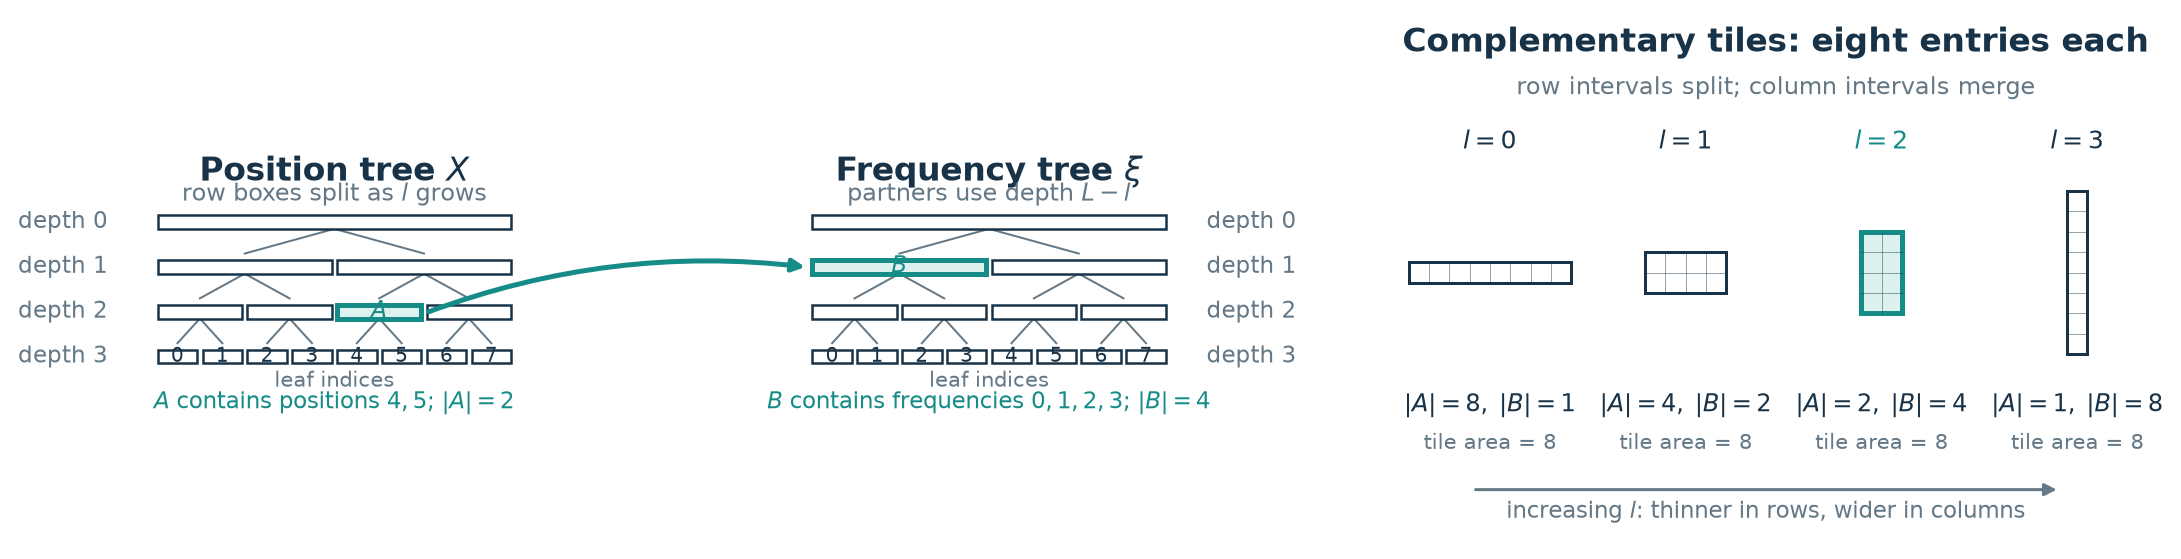
\includegraphics[width=\linewidth]{figures/two-trees.png}
\caption{The two binary trees and their complementary tilings. The selected pair has depths $\ell=2$ and $L-\ell=1$ for $L=3$. Row intervals split with depth; their column partners merge. Each displayed tile has eight entries, while its aspect ratio changes. The figure describes index geometry, not a general rank theorem.}
\label{fig:two-trees}
\end{figure}

Figure~\ref{fig:tiling} compares a fixed tiling with the middle complementary tiling at tolerance $10^{-6}$. The same kernel and same direct rank measurement lead to very different conclusions.

\begin{figure}[htbp]
\centering
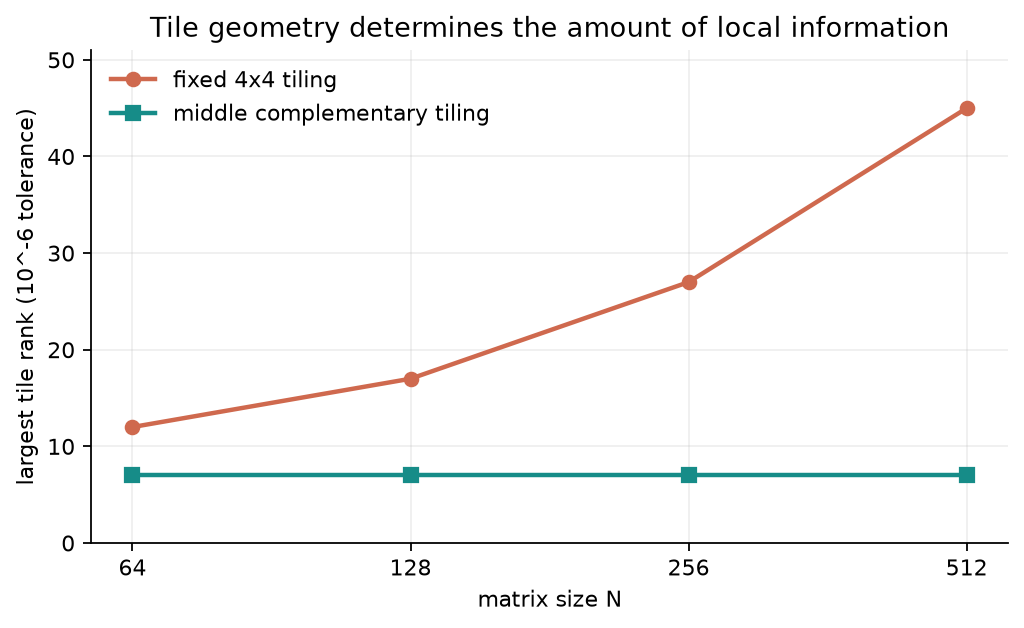
\includegraphics[width=0.87\linewidth]{figures/tile-ranks.png}
\caption{A bad tiling cannot always be repaired by a better compressor. Here the maximum rank grows with $N$ in a fixed $4\times4$ tiling but is nearly constant in a middle complementary tiling. Data: \texttt{results/butterfly-discovery-ranks.json}.}
\label{fig:tiling}
\end{figure}

\subsection{Representation first: local low rank is not yet a fast algorithm}
At the middle level, if $L$ is even, there are $N$ square tiles of size $\sqrt N\times\sqrt N$. One rank-$r$ tile has $O(r\sqrt N)$ leading factor entries; this is not an assertion that constructing it from the full tile costs only that much. Across all tiles, independent storage and apply work total
\begin{equation}
 N\times O(r\sqrt N)=O(rN^{3/2}).
 \label{eq:middlecost}
\end{equation}
This is \textbf{useful}: middle-level splits and low ranks are real. It is not yet $O(N\log N)$, because there are too many independent bases and local products. The paper responds by recursively factorizing the left and right bases, rather than doing more independent SVDs.

\subsection{Nesting gives speed}
Suppose two old summaries $c_1,c_2$ feed a new tile. Their contributions can be re-expressed in the new tile's small basis $U_{\rm new}$:
\begin{equation}
 U_1c_1+U_2c_2\approx U_{\rm new}(T_1c_1+T_2c_2).
 \label{eq:transfer}
\end{equation}
The small transfer matrices $T_1,T_2$ reuse earlier work instead of constructing a new summary from scratch. Repeating this relation through both trees yields nested bases and a ladder of sparse factors.

If old ranks are $r_0,r_1$ and the new rank is $r_2$, one merge has at most
\begin{equation}
 r_2(r_0+r_1)
 \label{eq:transfercost}
\end{equation}
stored entries before zero and identity entries are removed. With bounded ranks, $O(N)$ entries per stage and $O(\log N)$ stages give $O(N\log N)$ storage and apply work. This is the precise meaning of:
\takeaway{Tiles give low rank; nesting gives speed.}

Our small Python driver uses a one-sided column-ID version of this nesting. The reference paper's middle-out construction is more symmetric and contains the precise recursions. These two descriptions share structure but are not identical algorithms.

\subsection{Sampling and construction remain a separate budget}
Three access models deserve different cost estimates:
\begin{itemize}
 \item \textbf{All entries read.} Simple, deterministic and general. Reading a dense matrix already costs $\Theta(N^2)$. Our teaching/reference builder uses all rows of every tile; it is not the reference paper's optimal construction.
 \item \textbf{Black-box products.} Random probes against $K$ and $K^*$ identify local spaces. For an $N\times N$ matrix with bounded tile ranks, the paper's matrix-product construction has $O(N^{3/2}\log N)$ work when its required fast operator products have unit accounted cost \cite{li2015butterfly}.
 \item \textbf{Sampled entries.} Its sampled-entry route obtains $O(N^{3/2})$ construction under its coherence hypotheses. Row-sampled interpolative methods provide another route with a different access model \cite{pang2018idbf}.
\end{itemize}
The common grammar deliberately separates \textbf{representation} (what is stored) from \textbf{sampling} (how it is obtained). A fast apply does not automatically pay back an expensive construction.

\subsection{The FFT supplies an exact special case}
Let $N=2^L$ and $F_{jk}=e^{2\pi ijk/N}$. Choose residue classes
\[
j=a+2^\ell u,\qquad k=b+2^{L-\ell}v.
\]
Then
\[
\frac{jk}{N}
=\frac{ab}{N}+\frac{av}{2^\ell}+\frac{bu}{2^{L-\ell}}+uv.
\]
Because $uv\in\mathbb Z$, $\exp(2\pi iuv)=1$. Every complementary tile is \textbf{exactly} rank one: a tile constant, a row-only vector and a column-only vector. Bit reversal makes these residue classes contiguous. Reversing only one tree is insufficient.

This exact statement must not be confused with a numerical rank in another ordering. A contiguous natural-order tile is exactly full rank on its short side by a Vandermonde argument, although its short-arc Fourier nodes are ill conditioned: at $N=256$, its numerical $10^{-12}$-ranks across the stages are $1,2,4,8,11,8,4,2,1$. If one block is a residue class and the other is contiguous, the mixed matrix is a full Fourier block: at the middle of $N=1024$ both its exact and numerical ranks are $32$. Thus both-tree bit reversal creates an identity; one-sided reversal does not merely lose a constant factor.

For rank-one tiles, factors store $N$ at $W$, $2N$ at each of $L$ intermediate $G_\ell$, and $N$ at $U$. Therefore
\begin{equation}
 \nnz=2N\log_2N+2N.
 \label{eq:fftcount}
\end{equation}
Cooley--Tukey even/odd recombination supplies the actual FFT algorithm \cite{cooley1965fft}. With $E$ and $O$ the length-$N/2$ transforms of the even and odd inputs and $\omega_N=e^{2\pi i/N}$, the sign convention above gives
\begin{equation}
 (F_Ng)_j=E_j+\omega_N^jO_j,\qquad
 (F_Ng)_{j+N/2}=E_j-\omega_N^jO_j,
 \qquad 0\le j<N/2.
 \label{eq:cooley-tukey}
\end{equation}
Reusing the two half-transforms gives $T(N)=2T(N/2)+O(N)=O(N\log N)$. The residue identity supplies exact rank-one tiles; \eqref{eq:cooley-tukey} supplies the recursive algorithm. The count \eqref{eq:fftcount} describes the factor representation; an in-place FFT does not need to materialize the full factor chain.

\begin{figure}[htbp]
\centering
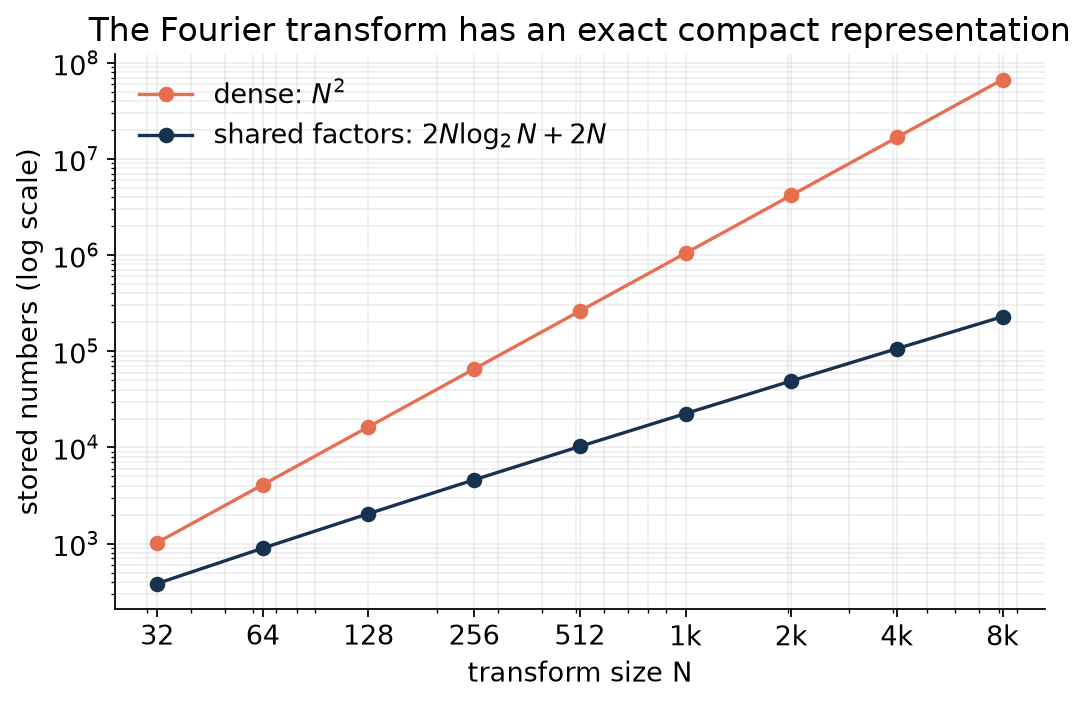
\includegraphics[width=0.82\linewidth]{figures/dft-storage.png}
\caption{Exact DFT factor storage compared with dense. Both Python and Rust independently check rank one at every stage and reconstruction of the underlying DFT operator.}
\label{fig:dftstorage}
\end{figure}
